\documentclass{ximera}[font=12pt]

%Next 2 lines create spaces between items in itemize and enumerate
\setitemize{itemsep=1.5ex}
\setenumerate{itemsep=1.5ex}

%Creates space between paragraphs - Maybe???
\setlength{\parskip}{\medskipamount}


\title{Adding Integers: Numberline}    % Use xmlatex all -s to compile when SERVE refuses to work.
\author{Kelly Stady}
\license{CC: 0}                        % replace with an appropriate license, or set it in xmPreamble

\begin{document}

\begin{abstract}

\end{abstract}

\maketitle
\label{xim:AddIntNumLActivity}


\section*{Adding Integers on a Number Line}

Another way to visualize addition is to add on a number line.  The steps are given below.


\begin{enumerate}
\item Locate the first number on the number line.

\item If the second number is \textbf{positive}, move to the \textbf{right} that many units.

\item If the second number is \textbf{negative}, take the absolute value of the number and move to the \textbf{left} that many units.
\end{enumerate}


\begin{example}
To find the value of $3+7,$ start at $3$ then move 7 units to the \textbf{right}.  
%Movement is to the right, since a \textbf{positive} number is added to 3.

~ \\[3em]  %Creates vertical space
\begin{tikzpicture}[x=0.75cm,>=latex] % Use latex arrowhead style
    \draw[thick, <->] (-6,0)--(11,0); % Number line from -6 to 11
    \foreach \x in {-5,...,10}
    \draw[shift={(\x,0)},color=black] (0pt,2pt) -- (0pt,-2pt) node[below] {\footnotesize $\x$};
    \fill (3,0) circle (1.8pt);
    \draw[->,out=60,in=120,color=glaucous, thick] (3,0) to (4,0) to (5,0) to (6,0) to (7,0) to (8,0) to (9,0) to (10,0); % Curves
    \node[color=red!65!black] at (10,-0.75) {\small \textbf{Stop}};
    \node[color=darkgreen] at (3,-0.75) {\small \textbf{Start}};
    \node at (6.5,0.9) {$3 + 7 = 10$};
\end{tikzpicture}
\end{example}

\begin{example}
To find the value of $3+(-7),$ start at $3$ then move $|-7| = 7$ units to the \textbf{left}.  
%Movement is to the left, since a \textbf{negative} number is added to 3.

~ \\[3em]
\begin{tikzpicture}[x=0.75cm,>=latex] % Use latex arrowhead style
%\begin{scope}[shift={(0, -4)}]
    \draw[thick, <->] (-6,0)--(11,0); % Number line from -6 to 11
    \foreach \x in {-5,...,10}
    \draw[shift={(\x,0)},color=black] (0pt,2pt) -- (0pt,-2pt) node[below] {\footnotesize $\x$}; % Tick marks for numbers
    \fill (3,0) circle (1.8pt); % Mark start at 3
    % Movement humps from 3 to -4
    \draw[<-,out=60,in=120,color=glaucous, thick] (-4,0) to (-3,0) to (-2,0) to (-1,0) to (0,0) to (1,0) to (2,0) to (3,0); % Curves
    \node[color=darkgreen] at (3,-0.75) {\small \textbf{Start}};
    \node[color=red!65!black] at (-4,-0.75) {\small \textbf{Stop}};
    \node at (-0.5,0.9) {$3 + (-7) = -4$}; % Label for the operation
%\end{scope}

\end{tikzpicture}

\end{example}

INSERT VIDEO HERE!!  %Add -4 + 5 and -2 + (-3)  show that it doesn't matter if we start at -4 or 5 - Commutative property of addition


\begin{problem}
Add using the number line shown below.

\[ -2 + 3 \begin{prompt}=\answer{1}\end{prompt}\]

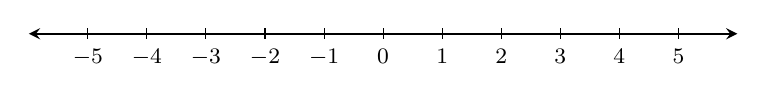
\begin{tikzpicture}[x=0.75cm,>=stealth]
        \draw[thick, <->] (-6,0)--(6,0);
        \foreach \x in {-5,...,5}
        \draw[shift={(\x,0)},color=black] (0pt,2pt) -- (0pt,-2pt) node[below] {\footnotesize $\x$};
\end{tikzpicture}

\end{problem}


\begin{problem}
Add using the number line shown below.

\[ -12 + (-3) \begin{prompt}=\answer{-15}\end{prompt} \]

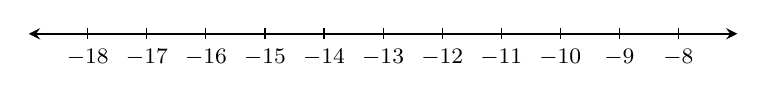
\begin{tikzpicture}[x=0.75cm,>=stealth]
        \draw[thick, <->] (-19,0)--(-7,0);
        \foreach \x in {-18,...,-8}
        \draw[shift={(\x,0)},color=black] (0pt,2pt) -- (0pt,-2pt) node[below] {\footnotesize $\x$};
\end{tikzpicture}

\end{problem}

\begin{problem}
Add using the number line shown below.

\[ -1 + 4 \begin{prompt}=\answer{3}\end{prompt} \]


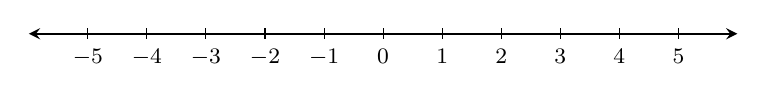
\begin{tikzpicture}[x=0.75cm,>=stealth]
        \draw[thick, <->] (-6,0)--(6,0);
        \foreach \x in {-5,...,5}
        \draw[shift={(\x,0)},color=black] (0pt,2pt) -- (0pt,-2pt) node[below] {\footnotesize $\x$};
\end{tikzpicture}

\end{problem}


\begin{problem}

Does the answer to the previous problem change if you switch the order of the numbers and find the value of $4 + (-1)?$

\begin{multipleChoice}
\choice[correct]{No.}
\choice{Yes.}
\end{multipleChoice}

\begin{feedback}[correct]
That's right, the answer does NOT change!  This is due to a property of addition called the Commutative Property.  
The \textbf{Commutative Property of Addition} states that numbers can be added in any order and the result will be the same.  Therefore, $-1 + 4 = 4 + (-1).$
\end{feedback}

\end{problem}

\end{document}

